% Steiner chain of 7 circles between two non-concentric circles (inverse of a concentric chain); tangencies checked to 1e-9.
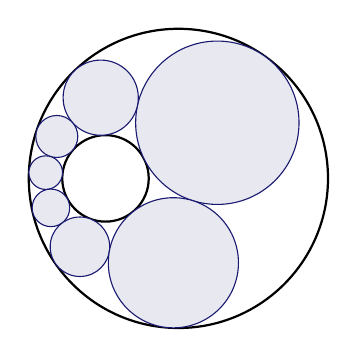
\begin{tikzpicture}
\draw[thick] (0.0000,0.0000) circle (1.9000);
\draw[thick] (-0.9258,0.0000) circle (0.5491);
\draw[MidnightBlue,fill=MidnightBlue!10] (0.4947,0.7066) circle (1.0374);
\draw[MidnightBlue,fill=MidnightBlue!10] (-0.9864,1.0249) circle (0.4775);
\draw[MidnightBlue,fill=MidnightBlue!10] (-1.5442,0.5321) circle (0.2667);
\draw[MidnightBlue,fill=MidnightBlue!10] (-1.6849,0.0730) circle (0.2135);
\draw[MidnightBlue,fill=MidnightBlue!10] (-1.6188,-0.3742) circle (0.2385);
\draw[MidnightBlue,fill=MidnightBlue!10] (-1.2503,-0.8682) circle (0.3778);
\draw[MidnightBlue,fill=MidnightBlue!10] (-0.0635,-1.0717) circle (0.8264);
\end{tikzpicture}
